\documentclass[a4paper]{article}
\usepackage[T1]{fontenc}
\usepackage[utf8]{inputenc}
\usepackage{lmodern}
\usepackage{amsmath,amssymb}
\usepackage[top=3cm,bottom=2cm,left=2cm,right=2cm]{geometry}
\usepackage{fancyhdr}
\usepackage{esvect,esint}
\usepackage{xcolor}
\usepackage{tikz}\usetikzlibrary{calc}

\parskip1em\parindent0pt\let\ds\displaystyle

\begin{document}

\pagestyle{fancy}
\fancyhf{}
\setlength{\headheight}{15pt}
\fancyhead[L]{Electromagnétisme}\fancyhead[R]{Question 45}

% Énoncé
\begin{center}
	\large{\boldmath{\textbf{Champ magnétique dans une bobine}}}
\end{center}

% Correction

On s'intéresse à une bobine infinie d'axe \(O\vv{z}\) parcourue par un courant orthoradial \(I\) dans chacune de ses spires et possédant une densité de spires \(n\).
On admet que le champ magnétique à l'extérieur de la bobine \(\vv{B_{\mathrm{ext}}}\) est nul :\begin{center}\fcolorbox{red}{white}{\(\vv{B_{\mathrm{ext}}}=\vv{0}\)}\end{center}
On se place en coordonnées cylindriques \(\vv{u_r},\vv{u_\theta},\vv{z}\).
Les plans \(z=\)cste sont plans de symétrie de la distribution de courant donc \(\vv{B_{\mathrm{int}}}\) leur est orthogonal.\\
Donc \(\vv{B_{\mathrm{int}}}=B_{\mathrm{int}}\vv{z}\).\\
La distribution de courant est invariante par translation selon \(z\) et par rotation selon \(\theta\) donc \(B_{\mathrm{int}}=B_{\mathrm{int}}(r)\).\\
Enfin, en appliquant le théorème de Stokes sur un carré de côté \(a\) :\begin{center}
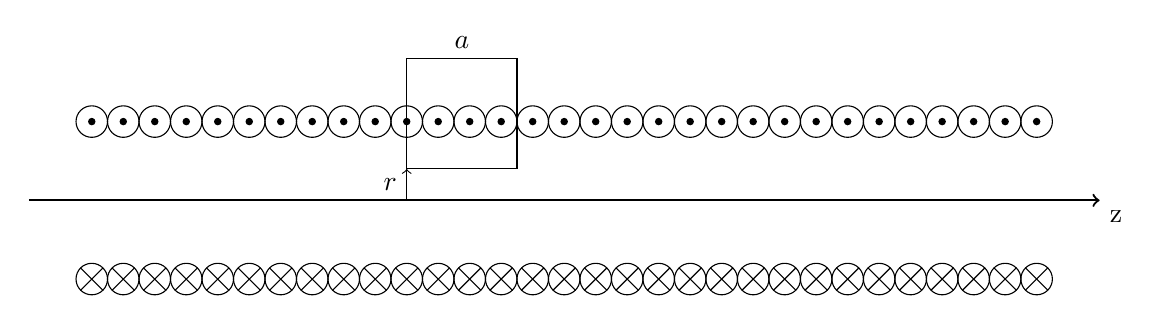
\begin{tikzpicture}[scale=.4]
    \draw[thick,->] (-2,2.5) to (32,2.5) node[anchor=north west]{z};
    \draw (10,3.5) rectangle (13.5,7);
    \draw (11.75,7) node[anchor=south]{\(a\)};
    \draw[->](10,2.5)to(10,3.5)node[anchor=north east]{\(\vv{r}\)};
    \foreach \x in {0,...,30}
        \draw (\x ,0) circle (0.5);
    \foreach \x in {0,...,30}
        \draw (\x ,5) circle (0.5);
    \foreach \x in {0,...,30}
        \filldraw[fill=black] (\x ,5) circle (0.1);
    \foreach \x in {0,...,30}
        \draw (\x -0.36,-0.36) to (\x +0.36,0.36);
    \foreach \x in {0,...,30}
        \draw (\x +0.36,-0.36) to (\x -0.36,0.36);
\end{tikzpicture}
\end{center}
On a \(aB_{\mathrm{int}}(r)=\mu_0nIa\) en tenant compte du fait que \(\vv{B_{\mathrm{ext}}}=\vv{0}\).
Donc \begin{center}\fcolorbox{red}{white}{\(\vv{B_{\mathrm{int}}}=\mu_0nI\vv{z}\)}\end{center}


\end{document}
